\chapter{Value methods}
\label{chap05}

\section{Return values}
\index{return}
\index{statement!return}
\index{value method}
\index{method!value}
\index{return value}
\index{void}
\index{method!void}

Some of the methods we have used, like the Math
functions, produce results.  That is, the effect of
invoking the method is to generate a new value, which we
usually assign to a variable or use as part of an expression.
For example:

\begin{code}
    double e = Math.exp(1.0);
    double height = radius * Math.sin(angle);
\end{code}

But so far all our methods have been {\bf void}; that is, methods
that return no value.  When you invoke a void method, it is typically
on a line by itself, with no assignment:

\begin{code}
    countdown(3);
    nLines(3);
\end{code}

In this chapter we write methods that return things, which I call
{\bf value} methods.  The first example is {\tt area}, which takes a
{\tt double} as a parameter, and returns the area of a circle with the
given radius:

\begin{code}
  public static double area(double radius) {
    double area = Math.PI * radius * radius;
    return area;
  }
\end{code}

The first thing you should notice is that the beginning of the
method definition is different.  Instead of {\tt public static
void}, which indicates a void method, we see {\tt public static
double}, which means that the return value from this method
is a {\tt double}.  I still haven't explained what
{\tt public static} means, but be patient.
\index{static}

The last line is a new form of the
{\tt return} statement that includes a return value.  This
statement means, ``return immediately from this method and
use the following expression as the return value.''  The
expression you provide can be arbitrarily complicated,
so we could have written this method more concisely:

\begin{code}
  public static double area(double radius) {
    return Math.PI * radius * radius;
  }
\end{code}

On the other hand, {\bf temporary} variables like {\tt area} often
make debugging easier.  In either case, the type of the expression in
the {\tt return} statement must match the return type of the method.
In other words, when you declare that the return type is {\tt double},
you are making a promise that this method will eventually
produce a {\tt double}.  If you try to {\tt return} with no
expression, or an expression with the wrong type, the compiler will
take you to task.

\index{temporary variable}
\index{variable!temporary}

Sometimes it is useful to have multiple return
statements, one in each branch of a conditional:

\begin{code}
  public static double absoluteValue(double x) {
    if (x < 0) {
      return -x;
    } else {
      return x;
    }
  }
\end{code}

Since these return statements are in an alternative conditional,
only one will be executed.  Although it is legal to have more than one
return statement in a method, you should keep in mind
that as soon as one is executed, the method
terminates without executing any subsequent statements.

Code that appears after a {\tt return} statement, or any place else
where it can never be executed, is called {\bf dead code}.  Some
compilers warn you if part of your code is dead.

\index{dead code}

If you put return statements inside a conditional, then
you have to guarantee that {\em every possible path} through
the program hits a return statement.  For example:

\begin{code}
  public static double absoluteValue(double x) {
    if (x < 0) {
      return -x;
    } else if (x > 0) {
      return x;
    }                          // WRONG!!
  }
\end{code}

This program is not legal because if {\tt x} is 0,
neither condition is true and the method ends without hitting
a return statement.  A typical compiler message would be ``return
statement required in absoluteValue,'' which is a confusing message
since there are already two of them.


\section{Program development}
\label{distance}
\index{program development}

At this point you should be able to look at complete Java methods and
tell what they do.  But it may not be clear yet how to go about
writing them.  I am going to suggest a method called {\bf incremental
  development}.
\index{incremental development}

As an example, imagine you want to find the distance between
two points, given by the coordinates $(x_1, y_1)$ and
$(x_2, y_2)$.  By the usual definition,

\begin{equation*}
distance = \sqrt{(x_2 - x_1)^2 +(y_2 - y_1)^2}
\end{equation*}

The first step is to consider what a {\tt distance} method
should look like in Java.  In other words, what are the inputs
(parameters) and what is the output (return value)?

In this case, the two points are the parameters, and it is
natural to represent them using four {\tt double}s, although
we will see later that there is a {\tt Point} object in Java
that we could use.  The return value is the distance, which
will have type {\tt double}.

Already we can write an outline of the method:

\begin{code}
  public static double distance
              (double x1, double y1, double x2, double y2) {
    return 0.0;
  }
\end{code}

The statement {\tt return 0.0;} is a place-keeper that is necessary
to compile the program.  Obviously, at this stage the
program doesn't do anything useful, but it is worthwhile to
try compiling it so we can identify any syntax errors before
we add more code.

To test the new method, we have to invoke it with
sample values.  Somewhere in {\tt main} I would add:

\begin{code}
    double dist = distance(1.0, 2.0, 4.0, 6.0);
\end{code}

I chose these values so that the horizontal
distance is 3 and the vertical distance is 4; that way,
the result will be 5 (the hypotenuse of a 3-4-5 triangle).
When you are testing a method, it is useful to know the right
answer.

Once we have checked the syntax of the method definition, we
can start adding lines of code one at a time.  After each
incremental change, we recompile and run the program.  If there is
an error at any point, we have a good idea where to look:
in the last line we added.

The next step is to find the differences
$x_2 - x_1$ and $y_2 - y_1$.  I store those values in
temporary variables named {\tt dx} and {\tt dy}.

\begin{code}
  public static double distance
              (double x1, double y1, double x2, double y2) {
    double dx = x2 - x1;
    double dy = y2 - y1;
    System.out.println("dx is " + dx);
    System.out.println("dy is " + dy);
    return 0.0;
  }
\end{code}

I added print statements so we can check the intermediate values
before proceeding.  They should be 3.0 and 4.0.

\index{scaffolding}

When the method is finished I remove the print statements.  Code
like that is called {\bf scaffolding}, because it is helpful for
building the program, but it is not part of the final product.

The next step is to square {\tt dx} and {\tt dy}.  We could use the
{\tt Math.pow} method, but it is simpler to multiply each term by
itself.

\begin{code}
  public static double distance
              (double x1, double y1, double x2, double y2) {
    double dx = x2 - x1;
    double dy = y2 - y1;
    double dsquared = dx*dx + dy*dy;
    System.out.println("dsquared is " + dsquared);
    return 0.0;
  }
\end{code}

Again, I would compile and run the program at this stage
and check the intermediate value (which should be 25.0).

Finally, we can use {\tt Math.sqrt} to compute and
return the result.

\begin{code}
  public static double distance
              (double x1, double y1, double x2, double y2) {
    double dx = x2 - x1;
    double dy = y2 - y1;
    double dsquared = dx*dx + dy*dy;
    double result = Math.sqrt(dsquared);
    return result;
  }
\end{code}

In {\tt main}, we can print and check the value of the result.

As you gain more experience programming, you might
write and debug more than one line at a time.  Nevertheless,
incremental development can save you a lot of time.
The key aspects of the process are:

\begin{itemize}

\item Start with a working program and make small, incremental
changes.  At any point, if there is an error, you will know
exactly where it is.

\item Use temporary variables to hold intermediate values so
you can print and check them.

\item Once the program is working, you can remove
scaffolding and consolidate multiple statements into
compound expressions, but only if it does not make the program
difficult to read.

\end{itemize}


\section{Composition}
\index{composition}

Once you define a new method,
you can use it as part of an expression, and you can build
new methods using existing methods.  For example, what if someone
gave you two points, the center of the circle and a point on
the perimeter, and asked for the area of the circle?

Let's say the center point is stored in the variables {\tt xc}
and {\tt yc}, and the perimeter point is in {\tt xp} and
{\tt yp}.  The first step is to find the radius of the circle, which
is the distance between the two points.  Fortunately, we have
a method, {\tt distance} that does that.

\begin{code}
    double radius = distance(xc, yc, xp, yp);
\end{code}

The second step is to find the area of a circle with that
radius, and return it.

\begin{code}
    double area = area(radius);
    return area;
\end{code}

Wrapping that all up in a method, we get:

\begin{code}
  public static double circleArea
              (double xc, double yc, double xp, double yp) {
    double radius = distance(xc, yc, xp, yp);
    double area = area(radius);
    return area;
  }
\end{code}

The temporary variables {\tt radius} and {\tt area} are
useful for development and debugging, but once the program is
working we can make it more concise by composing
the method invocations:

\begin{code}
  public static double circleArea
              (double xc, double yc, double xp, double yp) {
    return area(distance(xc, yc, xp, yp));
  }
\end{code}


\section{Overloading}
\label{overloading}
\index{overloading}

You might have noticed that {\tt circleArea}
and {\tt area} perform similar functions---finding
the area of a circle---but take different parameters.  For
{\tt area}, we have to provide the radius; for {\tt circleArea}
we provide two points.

If two methods do the same thing, it is natural to give them
the same name.
Having more than one method with the same name, which is called {\bf
overloading}, is legal in Java {\em as long as each version takes
different parameters}.  So we could rename {\tt circleArea}:

\begin{code}
  public static double area
              (double x1, double y1, double x2, double y2) {
    return area(distance(xc, yc, xp, yp));
  }
\end{code}

When you invoke an overloaded method, Java knows which version you
want by looking at the arguments that you provide.  If you write:

\begin{code}
    double x = area(3.0);
\end{code}

Java goes looking for a method named {\tt area} that
takes one {\tt double} as an argument, and so it uses the
first version, which interprets the argument as a radius.
If you write:

\begin{code}
    double x = area(1.0, 2.0, 4.0, 6.0);
\end{code}

Java uses the second version of {\tt area}.  And notice that the
second version of {\tt area} actually invokes the first.

Many Java methods are overloaded, meaning that there
are different versions that accept different numbers or types of
parameters.  For example, there are versions of {\tt print} and {\tt
println} that accept a single parameter of any type.  In the Math
class, there is a version of {\tt abs} that works on {\tt double}s,
and there is also a version for {\tt int}s.

Although overloading is a useful feature, it should be used
with caution.  You might get yourself nicely confused if you
are trying to debug one version of a method while accidently
invoking a different one.

And that reminds me of one of the cardinal rules of
debugging: {\bf make sure that the version of the program
you are looking at is the version of the program that is running!}

Some day you may find yourself making one change after another
in your program, and seeing the same thing every time you run it.
This is a warning sign that you are
not running the version of the program you think you are.  To
check, add a {\tt print} statement (it doesn't matter what
you print) and make sure the behavior of the program changes
accordingly.


\section{Boolean expressions}
\index{boolean}
\index{expression!boolean}

Most of the operations we have seen produce results that are
the same type as their operands.  For example, the {\tt +} operator
takes two {\tt int}s and produces an {\tt int}, or two {\tt double}s
and produces a {\tt double}, etc.

\index{operator!relational}
\index{relational operator}

The exceptions we have seen are the {\bf relational operators}, which
compare {\tt int}s and {\tt float}s and return either {\tt true} or
{\tt false}.  {\tt true} and {\tt false} are special values in Java,
and together they make up a type called {\bf boolean}.  You might
recall that when I defined a type, I said it was a set of values.  In
the case of {\tt int}s, {\tt double}s and {\tt String}s, those sets
are pretty big.  For {\tt boolean}s, there are only two values.

Boolean expressions and variables work just like other types of
expressions and variables:

\begin{code}
    boolean flag;
    flag = true;
    boolean testResult = false;
\end{code}

The first example is a simple variable declaration;
the second example is an assignment, and the third example is an
initialization.

The values {\tt true} and {\tt false}
are keywords in Java, so they may appear in a different color,
depending on your development environment.

\index{initialization}
\index{statement!initialization}

The result of a conditional operator is a boolean,
so you can store the result of a comparison in a variable:

\begin{code}
    boolean evenFlag = (n%2 == 0);     // true if n is even
    boolean positiveFlag = (x > 0);    // true if x is positive
\end{code}

and then use it as part of a conditional statement later:

\begin{code}
    if (evenFlag) {
      System.out.println("n was even when I checked it");
    }
\end{code}

A variable used in this way is called a {\bf flag}
because it flags the presence or absence of some condition.


\section{Logical operators}
\index{logical operator}
\index{operator!logical}

There are three {\bf logical operators} in Java: AND, OR and NOT,
which are denoted by the symbols {\tt \&\&}, {\tt ||} and
{\tt !}.  The semantics of these operators is similar
to their meaning in English.  For example {\tt x > 0 \&\& x < 10}
is true only if {\tt x} is greater than zero AND less than 10.
\index{semantics}

{\tt evenFlag || n\%3 == 0} is true if {\em either} of
the conditions is true, that is, if {\tt evenFlag} is true OR the
number is divisible by 3.

Finally, the NOT operator inverts a boolean expression, so {\tt
  !evenFlag} is true if {\tt evenFlag} is false---if the number is
odd.

\index{nested structure}

Logical operators can simplify nested
conditional statements.  For example, can you re-write
this code using a single conditional?

\begin{code}
    if (x > 0) {
      if (x < 10) {
        System.out.println("x is a positive single digit.");
      }
    }
\end{code}


\section{Boolean methods}
\label{boolean}
\index{boolean}
\index{method!boolean}

Methods can return boolean values just like any other type,
which is often convenient for hiding tests inside
methods.  For example:

\begin{code}
  public static boolean isSingleDigit(int x) {
    if (x >= 0 && x < 10) {
      return true;
    } else {
      return false;
    }
  }
\end{code}

The name of this method is {\tt isSingleDigit}.  It is common
to give boolean methods names that sound like yes/no questions.
The return type is {\tt boolean}, which means that every return
statement has to provide a boolean expression.

The code itself is straightforward, although it is longer than
it needs to be.  Remember that the expression {\tt x >= 0 \&\& x < 10}
has type boolean, so there is nothing wrong with returning it
directly and avoiding the {\tt if} statement altogether:

\begin{code}
  public static boolean isSingleDigit(int x) {
    return (x >= 0 && x < 10);
  }
\end{code}

In {\tt main} you can invoke this method in the usual ways:

\begin{code}
  boolean bigFlag = !isSingleDigit(17);
  System.out.println(isSingleDigit(2));
\end{code}

The first line sets {\tt bigFlag} to {\tt true}
only if 17 is {\em not} a single-digit number.  The second
line prints {\tt true} because 2 is a single-digit number.

The most common use of boolean methods is inside conditional
statements

\begin{code}
    if (isSingleDigit(x)) {
      System.out.println("x is little");
    } else {
      System.out.println("x is big");
    }
\end{code}


\section{More recursion}
\index{recursion}
\index{language!complete}
\index{factorial}
\label{factorial}

Now that we have methods that return values, we have a {\bf Turing
  complete} programming language, which means that we can compute
anything computable, for any reasonable definition of ``computable.''
\index{Turing, Alan}
\index{Church, Alonzo}
%
This idea was developed by Alonzo Church and Alan Turing, so it is
known as the Church-Turing thesis.  You can read more about it at
\url{http://en.wikipedia.org/wiki/Turing_thesis}.

To give you an idea of what you can do with the tools we have learned,
let's look at some methods for evaluating recursively-defined
mathematical functions.  A recursive definition is similar to a
circular definition, in the sense that the definition contains a
reference to the thing being defined.  A truly circular definition is
not very useful:

\begin{description}

\item[recursive:] an adjective used to describe a method that is recursive.

\end{description}

If you saw that definition in the dictionary, you might be
annoyed.  On the other hand, if you looked up the definition
of the mathematical function {\bf factorial}, you might
get something like:

\begin{eqnarray*}
&&  0! = 1 \\
&&  n! = n \cdot(n-1)!
\end{eqnarray*}

(Factorial is usually denoted with the symbol $!$, which is
not to be confused with the logical operator {\tt !} which
means NOT.)  This definition says that the factorial of 0 is 1,
and the factorial of any other value, $n$, is $n$ multiplied
by the factorial of $n-1$.  So $3!$ is 3 times $2!$, which is 2 times
$1!$, which is 1 times $0!$.  Putting it all together, we get
$3!$ equal to 3 times 2 times 1 times 1, which is 6.

If you can write a recursive definition of something, you can usually
write a Java method to evaluate it.  The first step is to decide what
the parameters are and what the return type is.  Since factorial is
defined for integers, the method takes an
integer as a parameter and returns an integer:

\begin{code}
  public static int factorial(int n) {
  }
\end{code}

\noindent If the argument happens to be zero, return 1:

\begin{code}
  public static int factorial(int n) {
    if (n == 0) {
      return 1;
    }
  }
\end{code}

That's the base case.

Otherwise, and this is the interesting part, we have to make
a recursive call to find the factorial of $n-1$, and then
multiply it by $n$.

\begin{code}
  public static int factorial(int n) {
    if (n == 0) {
      return 1;
    } else {
      int recurse = factorial(n-1);
      int result = n * recurse;
      return result;
    }
  }
\end{code}

The flow of execution for this program is similar to {\tt countdown}
from Section~\ref{recursion}.
If we invoke {\tt factorial} with the value 3:

Since 3 is not zero, we take the second branch and calculate
the factorial of $n-1$...

\begin{quote}
Since 2 is not zero, we take the second branch and calculate
the factorial of $n-1$...

\begin{quote}
Since 1 is not zero, we take the second branch and calculate
the factorial of $n-1$...

\begin{quote}
Since 0 {\em is} zero, we take the first branch and return
the value 1 immediately without making any more recursive
invocations.

\end{quote}

The return value (1) gets multiplied by {\tt n}, which is 1,
and the result is returned.

\end{quote}

The return value (1) gets multiplied by {\tt n}, which is 2,
and the result is returned.

\end{quote}

\noindent The return value (2) gets multiplied by {\tt n}, which is 3,
and the result, 6, is returned to {\tt main}, or whoever
invoked {\tt factorial(3)}.

\index{stack}
\index{diagram!state}
\index{diagram!stack}

Here is what the stack diagram looks like for this sequence of
method invocations:

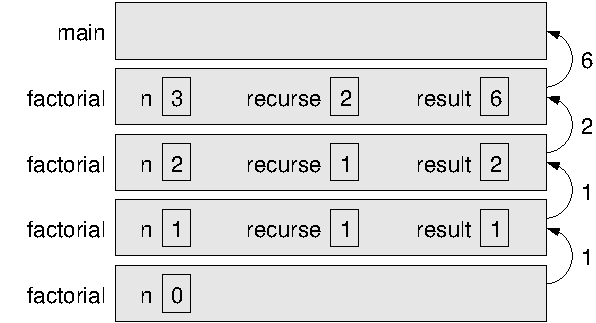
\includegraphics{figs/stack3.pdf}

The return values are shown being passed back up the stack.

Notice that in the last frame {\tt recurse} and {\tt result} do not
exist because when {\tt n=0} the branch that creates them does not
execute.


\section{Leap of faith}
\label{leap of faith}
\index{leap of faith}

Following the flow of execution is one way to read programs, but it can
quickly become disorienting.  An alternative is what I call the ``leap
of faith.''  When you come to a method invocation, instead of
following the flow of execution, you {\em assume} that the method
works correctly and returns the appropriate value.

In fact, you are already practicing this leap of faith
when you use Java methods.  When you invoke {\tt Math.cos}
or {\tt System.out.println}, you don't examine the implementations of
those methods.  You just assume that they work.

You can apply the same logic to your own methods.
For example, in Section~\ref{boolean} we wrote a method called
{\tt isSingleDigit} that determines whether a number is between
0 and 9.  Once we convince ourselves that this method
is correct---by testing and examination of the code---we can
use the method without ever looking at the code again.

The same is true of recursive programs.  When you get to
the recursive invocation, instead of following the flow of
execution, you should {\em assume} that the recursive invocation
works, and then ask yourself,
``Assuming that I can find the factorial of $n-1$, can I
compute the factorial of $n$?''  Yes, you can, by multiplying by $n$.

Of course, it is strange to assume that the method
works correctly when you have not even finished writing it,
but that's why it's called a leap of faith!


\section{One more example}
\index{fibonacci}
\label{fibonacci}

The second most common example of a recursively-defined
mathematical function is {\tt fibonacci}, which has the
following definition:

\begin{eqnarray*}
&& fibonacci(0) = 1 \\
&& fibonacci(1) = 1 \\
&& fibonacci(n) = fibonacci(n-1) + fibonacci(n-2);
\end{eqnarray*}

Translated into Java, this is

\begin{code}
  public static int fibonacci(int n) {
    if (n == 0 || n == 1) {
      return 1;
    } else {
      return fibonacci(n-1) + fibonacci(n-2);
    }
  }
\end{code}

If you try to follow the flow of execution here, even for small
values of {\tt n}, your head explodes.  But according to the leap of
faith, if we assume that the two recursive invocations work correctly, then
it is clear that we get the right result by adding them together.


\section{Glossary}

\begin{description}

\item[return type:]  The part of a method declaration that indicates
what type of value the method returns.

\item[return value:]  The value provided as the result of a method
invocation.

\item[dead code:]  Part of a program that can never be executed,
often because it appears after a {\tt return} statement.

\item[scaffolding:]  Code that is used during program development
but is not part of the final version.

\item[void:]  A special return type that indicates a void method;
that is, one that does not return a value.

\item[overloading:]  Having more than one method with the same name
but different parameters.  When you invoke an overloaded method,
Java knows which version to use by looking at the arguments you
provide.

\item[boolean:]  A type of variable that can contain only the two
values {\tt true} and {\tt false}.

\item[flag:]  A variable (usually {\tt boolean}) that records
a condition or status information.

\item[conditional operator:]  An operator that compares two values
and produces a boolean that indicates the relationship between the
operands.

\item[logical operator:]  An operator that combines boolean values
and produces boolean values.

\index{return type}
\index{return value}
\index{dead code}
\index{scaffolding}
\index{void}
\index{overloading}
\index{boolean}
\index{operator!conditional}
\index{operator!logical}


\end{description}


\section{Exercises}

\begin{exercise}
\label{ex.isdiv}

Write a method named {\tt isDivisible} that takes
two integers, {\tt n} and {\tt m} and that returns {\tt true}
if {\tt n} is divisible by {\tt m} and {\tt false} otherwise.

\end{exercise}


\begin{exercise}
\label{ex.multadd}

Many computations can be expressed concisely using the ``multadd''
operation, which takes three operands and computes {\tt a*b + c}.  Some
processors even provide a hardware implementation of this operation for
floating-point numbers.

\begin{enumerate}

\item Create a new program called {\tt Multadd.java}.

\item Write a method called {\tt multadd} that takes three {\tt doubles}
as parameters and that returns their multadditionization.

\item Write a {\tt main} method that tests {\tt multadd} by invoking it with a
few simple parameters, like {\tt 1.0, 2.0, 3.0}.

\item Also in {\tt main}, use {\tt multadd} to compute the
following values:

\begin{eqnarray*}
& \sin \frac{\pi}{4} + \frac{\cos \frac{\pi}{4}}{2} & \\
& \log 10 + \log 20 &
\end{eqnarray*}

\item Write a method called {\tt yikes} that takes a
double as a parameter and that uses {\tt multadd} to calculate

\begin{eqnarray*}
x e^{-x} + \sqrt{1 - e^{-x}}
\end{eqnarray*}

HINT: the Math method for raising $e$ to a power is {\tt Math.exp}.

\end{enumerate}

In the last part, you get a chance to write a method that invokes
a method you wrote.  Whenever you do that, it is a good idea to
test the first method carefully before you start working on the
second.  Otherwise, you might find yourself debugging two methods
at the same time, which can be difficult.

One of the purposes of this exercise is to practice pattern-matching:
the ability to recognize a specific problem as an instance of a
general category of problems.

\end{exercise}


\begin{exercise}
If you are given three sticks, you may or may not be able to arrange
them in a triangle.  For example, if one of the sticks is 12 inches
long and the other two are one inch long, you will
not be able to get the short sticks to meet in the middle.  For any
three lengths, there is a simple test to see if it is possible to form
a triangle:

\begin{quotation}
``If any of the three lengths is greater than the sum of the other two,
then you cannot form a triangle.  Otherwise, you can.''
\end{quotation}

Write a method named {\tt isTriangle} that it takes three integers as
arguments, and that returns either {\tt true} or {\tt false},
depending on whether you can or cannot form a triangle from sticks
with the given lengths.

The point of this exercise is to use conditional statements to
write a value method.

\end{exercise}


\begin{exercise}
What is the output of the following program?  The purpose of
this exercise is to make sure you understand logical operators
and the flow of execution through value methods.

\begin{code}
  public static void main(String[] args) {
      boolean flag1 = isHoopy(202);
      boolean flag2 = isFrabjuous(202);
      System.out.println(flag1);
      System.out.println(flag2);
      if (flag1 && flag2) {
          System.out.println("ping!");
      }
      if (flag1 || flag2) {
          System.out.println("pong!");
      }
  }

  public static boolean isHoopy(int x) {
      boolean hoopyFlag;
      if (x%2 == 0) {
          hoopyFlag = true;
      } else {
          hoopyFlag = false;
      }
      return hoopyFlag;
  }

  public static boolean isFrabjuous(int x) {
      boolean frabjuousFlag;
      if (x > 0) {
          frabjuousFlag = true;
      } else {
          frabjuousFlag = false;
      }
      return frabjuousFlag;
  }
\end{code}
\end{exercise}



\begin{exercise}
The distance between two points $(x_1, y_1)$ and $(x_2, y_2)$ is

\[ Distance = \sqrt{(x_2 - x_1)^2 +(y_2 - y_1)^2} \]

Write a method named {\tt distance} that takes four
doubles as parameters---{\tt x1}, {\tt y1}, {\tt x2} and {\tt
y2}---and that prints the distance between the points.

You should assume that there is a method named {\tt sumSquares}
that calculates and returns the sum of the squares of its arguments.
For example:

\begin{code}
    double x = sumSquares(3.0, 4.0);
\end{code}

would assign the value {\tt 25.0} to {\tt x}.

The point of this exercise is to write a new method that uses an
existing one.  You should write only one method: {\tt distance}.  You
should not write {\tt sumSquares} or {\tt main} and you should not
invoke {\tt distance}.
\end{exercise}


\begin{exercise}
The point of this exercise is to use a stack diagram to understand
the execution of a recursive program.

\begin{code}
public class Prod {

    public static void main(String[] args) {
        System.out.println(prod(1, 4));
    }

    public static int prod(int m, int n) {
        if (m == n) {
            return n;
        } else {
            int recurse = prod(m, n-1);
            int result = n * recurse;
            return result;
        }
    }
}
\end{code}

\begin{enumerate}

\item Draw a stack diagram showing the state of the program just
before the last instance of {\tt prod} completes.
What is the output of this program?

\item Explain in a few words what {\tt prod} does.

\item Rewrite {\tt prod} without using the temporary variables
{\tt recurse} and {\tt result}.

\end{enumerate}
\end{exercise}


\begin{exercise}
The purpose of this exercise is to translate a recursive definition
into a Java method.  The Ackerman function is defined for non-negative
integers as follows:

\begin{eqnarray}
A(m, n) = \begin{cases}
              n+1 & \mbox{if } m = 0 \\
        A(m-1, 1) & \mbox{if } m > 0 \mbox{ and } n = 0 \\
A(m-1, A(m, n-1)) & \mbox{if } m > 0 \mbox{ and } n > 0.
\end{cases}
\end{eqnarray}

Write a method called {\tt ack} that takes two {\tt int}s as
parameters and that computes and returns the value
of the Ackerman function.

Test your implementation of Ackerman by invoking it
from {\tt main} and printing the return value.

WARNING: the return value gets very big very quickly.  You should try it
only for small values of $m$ and $n$ (not bigger than 2).

\end{exercise}


\begin{exercise}
\begin{enumerate}

\item Create a program called {\tt Recurse.java} and
type in the following methods:

\begin{code}
    // first: returns the first character of the given String
    public static char first(String s) {
        return s.charAt(0);
    }

    // last: returns a new String that contains all but the
    // first letter of the given String
    public static String rest(String s) {
        return s.substring(1, s.length());
    }

    // length: returns the length of the given String
    public static int length(String s) {
        return s.length();
    }
\end{code}

\item Write some code in {\tt main} that tests each of these
methods.  Make sure they work, and make sure you understand
what they do.

\item Write a method called {\tt printString} that takes a
String as a parameter and that prints the letters of the
String, one on each line.  It should be a {\tt void} method.

\item Write a method called {\tt printBackward} that does
the same thing as {\tt printString} but that prints the String
backward (one character per line).

\item Write a method called {\tt reverseString} that takes
a String as a parameter and that returns a new String as a
return value.  The new String should contain the same letters
as the parameter, but in reverse order.  For example, the
output of the following code

\begin{code}
    String backwards = reverseString("Allen Downey");
    System.out.println(backwards);
\end{code}

should be

\begin{stdout}
yenwoD nellA
\end{stdout}

\end{enumerate}
\end{exercise}


\begin{exercise}
\label{ex.power}
Write a recursive method called {\tt power} that
takes a double {\tt x} and an integer {\tt n} and that
returns $x^n$.

Hint: a recursive definition of this
operation is $x^n = x \cdot x^{n-1}$.
Also, remember that anything raised to the zeroeth power
is 1.

Optional challenge: you can make this method more efficient, when {\tt
  n} is even, using $x^n = \left( x^{n/2} \right)^2$.

\end{exercise}


\begin{exercise}
\label{gcd}
(This exercise is based on page 44 of Ableson and Sussman's
{\em Structure and Interpretation of Computer Programs}.)

The following technique is known as Euclid's Algorithm because
it appears in Euclid's {\em Elements} (Book 7, ca.~300 BC).
It may be the oldest nontrivial algorithm\footnote{For a definition
of ``algorithm'', jump ahead to Section~\ref{algorithm}.}.

The process is based on the observation that, if $r$ is the
remainder when $a$ is divided by $b$, then the common divisors
of $a$ and $b$ are the same as the common divisors of $b$ and $r$.
Thus we can use the equation

\[ gcd(a, b) = gcd(b, r) \]

to successively reduce the problem of computing a GCD to the
problem of computing the GCD of smaller and smaller pairs of integers.
For example,

\[ gcd(36, 20) = gcd(20, 16) = gcd(16, 4) = gcd(4, 0) = 4 \]

implies that the GCD of 36 and 20 is 4.  It can be shown
that for any two starting numbers, this repeated reduction eventually
produces a pair where the second number is 0.  Then the GCD is the
other number in the pair.

Write a method called {\tt gcd} that takes two integer parameters and
that uses Euclid's algorithm to compute and return the greatest
common divisor of the two numbers.
\end{exercise}


